\let\negmedspace\undefined
\let\negthickspace\undefined
\documentclass[journal]{IEEEtran}
\usepackage[a5paper, margin=10mm, onecolumn]{geometry}
%\usepackage{lmodern} 
\usepackage{tfrupee} 

\setlength{\headheight}{1cm} 
\setlength{\headsep}{0mm}     

\usepackage{gvv-book}
\usepackage{gvv}
\usepackage{cite}
\usepackage{amsmath,amssymb,amsfonts,amsthm}
\usepackage{algorithmic}
\usepackage{graphicx}
\usepackage{textcomp}
\usepackage{xcolor}
\usepackage{txfonts}
\usepackage{listings}
\usepackage{enumitem}
\usepackage{mathtools}
\usepackage{gensymb}
\usepackage{comment}
\usepackage[breaklinks=true]{hyperref}
\usepackage{tkz-euclide} 
\usepackage{listings}                                        
\def\inputGnumericTable{}                                 
\usepackage[latin1]{inputenc}                                
\usepackage{color}                                            
\usepackage{array}                                            
\usepackage{longtable}                                       
\usepackage{calc}                                             
\usepackage{multirow}                                         
\usepackage{hhline}                                           
\usepackage{ifthen}                                           
\usepackage{lscape}

\begin{document}

\bibliographystyle{IEEEtran}
\vspace{3cm}

\title{5.2.70}
\author{AI25BTECH11003 - Bhavesh Gaikwad}
{\let\newpage\relax\maketitle}

\renewcommand{\thefigure}{\theenumi}
\renewcommand{\thetable}{\theenumi}
\setlength{\intextsep}{10pt} 


\numberwithin{equation}{enumi}
\numberwithin{figure}{enumi}
\renewcommand{\thetable}{\theenumi}


\textbf{Question}: 
For which values of p does the pair of equations given below have a unique solution.
\begin{center}
4x + py + 8 = 0 \\
2x + 2y + 2 = 0 
\end{center}

\textbf{Solution:}\\
Given:
\begin{align}
4x + py + 8 &= 0 \\
2x + 2y + 2 &= 0
\end{align}

Standard Form: $ \vec{A}\vec{x} = \vec{b} $ where:\\\\
Coefficient Matrix: $ \vec{A} = \myvec{4 & p \\ 2 & 2} $\\\\
Constant Vector: $ \vec{b} = \myvec{-8 \\ -2} $\\\\
Augmented Matrix: $ [\vec{A}|\vec{b}] = \myvec{4 & p & -8 \\ 2 & 2 & -2} $\\\\



For Unique Solution:\\
Unique Solution: $ \rank(\vec{A}) = \rank([\vec{A}|\vec{b}]) = n $ (number of variables)\\
For our system: $ n = 2 $ variables\\\\

Finding $\rank(\vec{A})$ - Rank of Coefficient Matrix\\

Initial Matrix $ \vec{A} $:
\begin{equation}
\vec{A} = \myvec{4 & p \\ 2 & 2}
\end{equation}

Row Operations on $\vec{A}$:
\begin{align}
R_2 &\to R_2 - \frac{1}{2}R_1
\end{align}

Row Echelon Form of $ \vec{A} $:
\begin{equation}
\myvec{4 & p \\ 0 & 2 - \tfrac{p}{2}}
\end{equation}\\\\

Rank Analysis:\\
    Case 1: If $ 2 - \dfrac{p}{2} \neq 0 $ (i.e., $ p \neq 4 $)\\
        Both rows are non-zero and linearly independent \\
        $ \Rightarrow \rank(\vec{A}) = 2 $\\\\
Case 2: If $ 2 - \dfrac{p}{2} = 0 $ (i.e., $ p = 4 $)\\
        Second row is zero, only first row is non-zero \\
        $ \Rightarrow \rank(\vec{A}) = 1 $
\bigskip

Finding $\rank([\vec{A}|\vec{b}])$ - Rank of Augmented Matrix

Initial Augmented Matrix:
\begin{equation}
\myvec{4 & p & -8 \\ 2 & 2 & -2}
\end{equation}

Row Operation on $[\vec{A}|\vec{b}]$:\\ 
\begin{align}
R_2 \to R_2 - \frac{1}{2}R_1
\end{align}

Row Echelon Form of Augmented Matrix:
\begin{equation}
\myvec{4 & p & -8 \\ 0 & 2-\frac{p}{2} & 2}
\end{equation}

Rank Analysis:\\
Case 1: If $ p \neq 4 $:\\
$\Rightarrow \rank([\vec{A}|\vec{b}]) = 2$\\

Case 2: If $ p = 4 $:\\
$ \Rightarrow \rank([\vec{A}|\vec{b}]) = 2 $\\\\

\bigskip

Comparing Ranks and Providing Solution Type
\begin{center}
\begin{tabular}[12pt]{ |c| c|}
    \hline
    \textbf{Variable} & \textbf{value}\\ 
    \hline
    \textbf{$A$} & $\myvec{1\\-3}$\\
    \hline
 \textbf{$B$} & $\myvec{4\\p}$\\
    \hline
 \textbf{$C$} & $\myvec{-9\\7}$\\
    \hline
    \end{tabular}
\end{center}

\begin{align}
\boxed{\therefore \, \text{For p} \, \epsilon \, \mathbb{R}-\{4\}, \, \text{the pair of equations has an Unique Solution.}}
\end{align}


\begin{figure}[htbp]
\centering
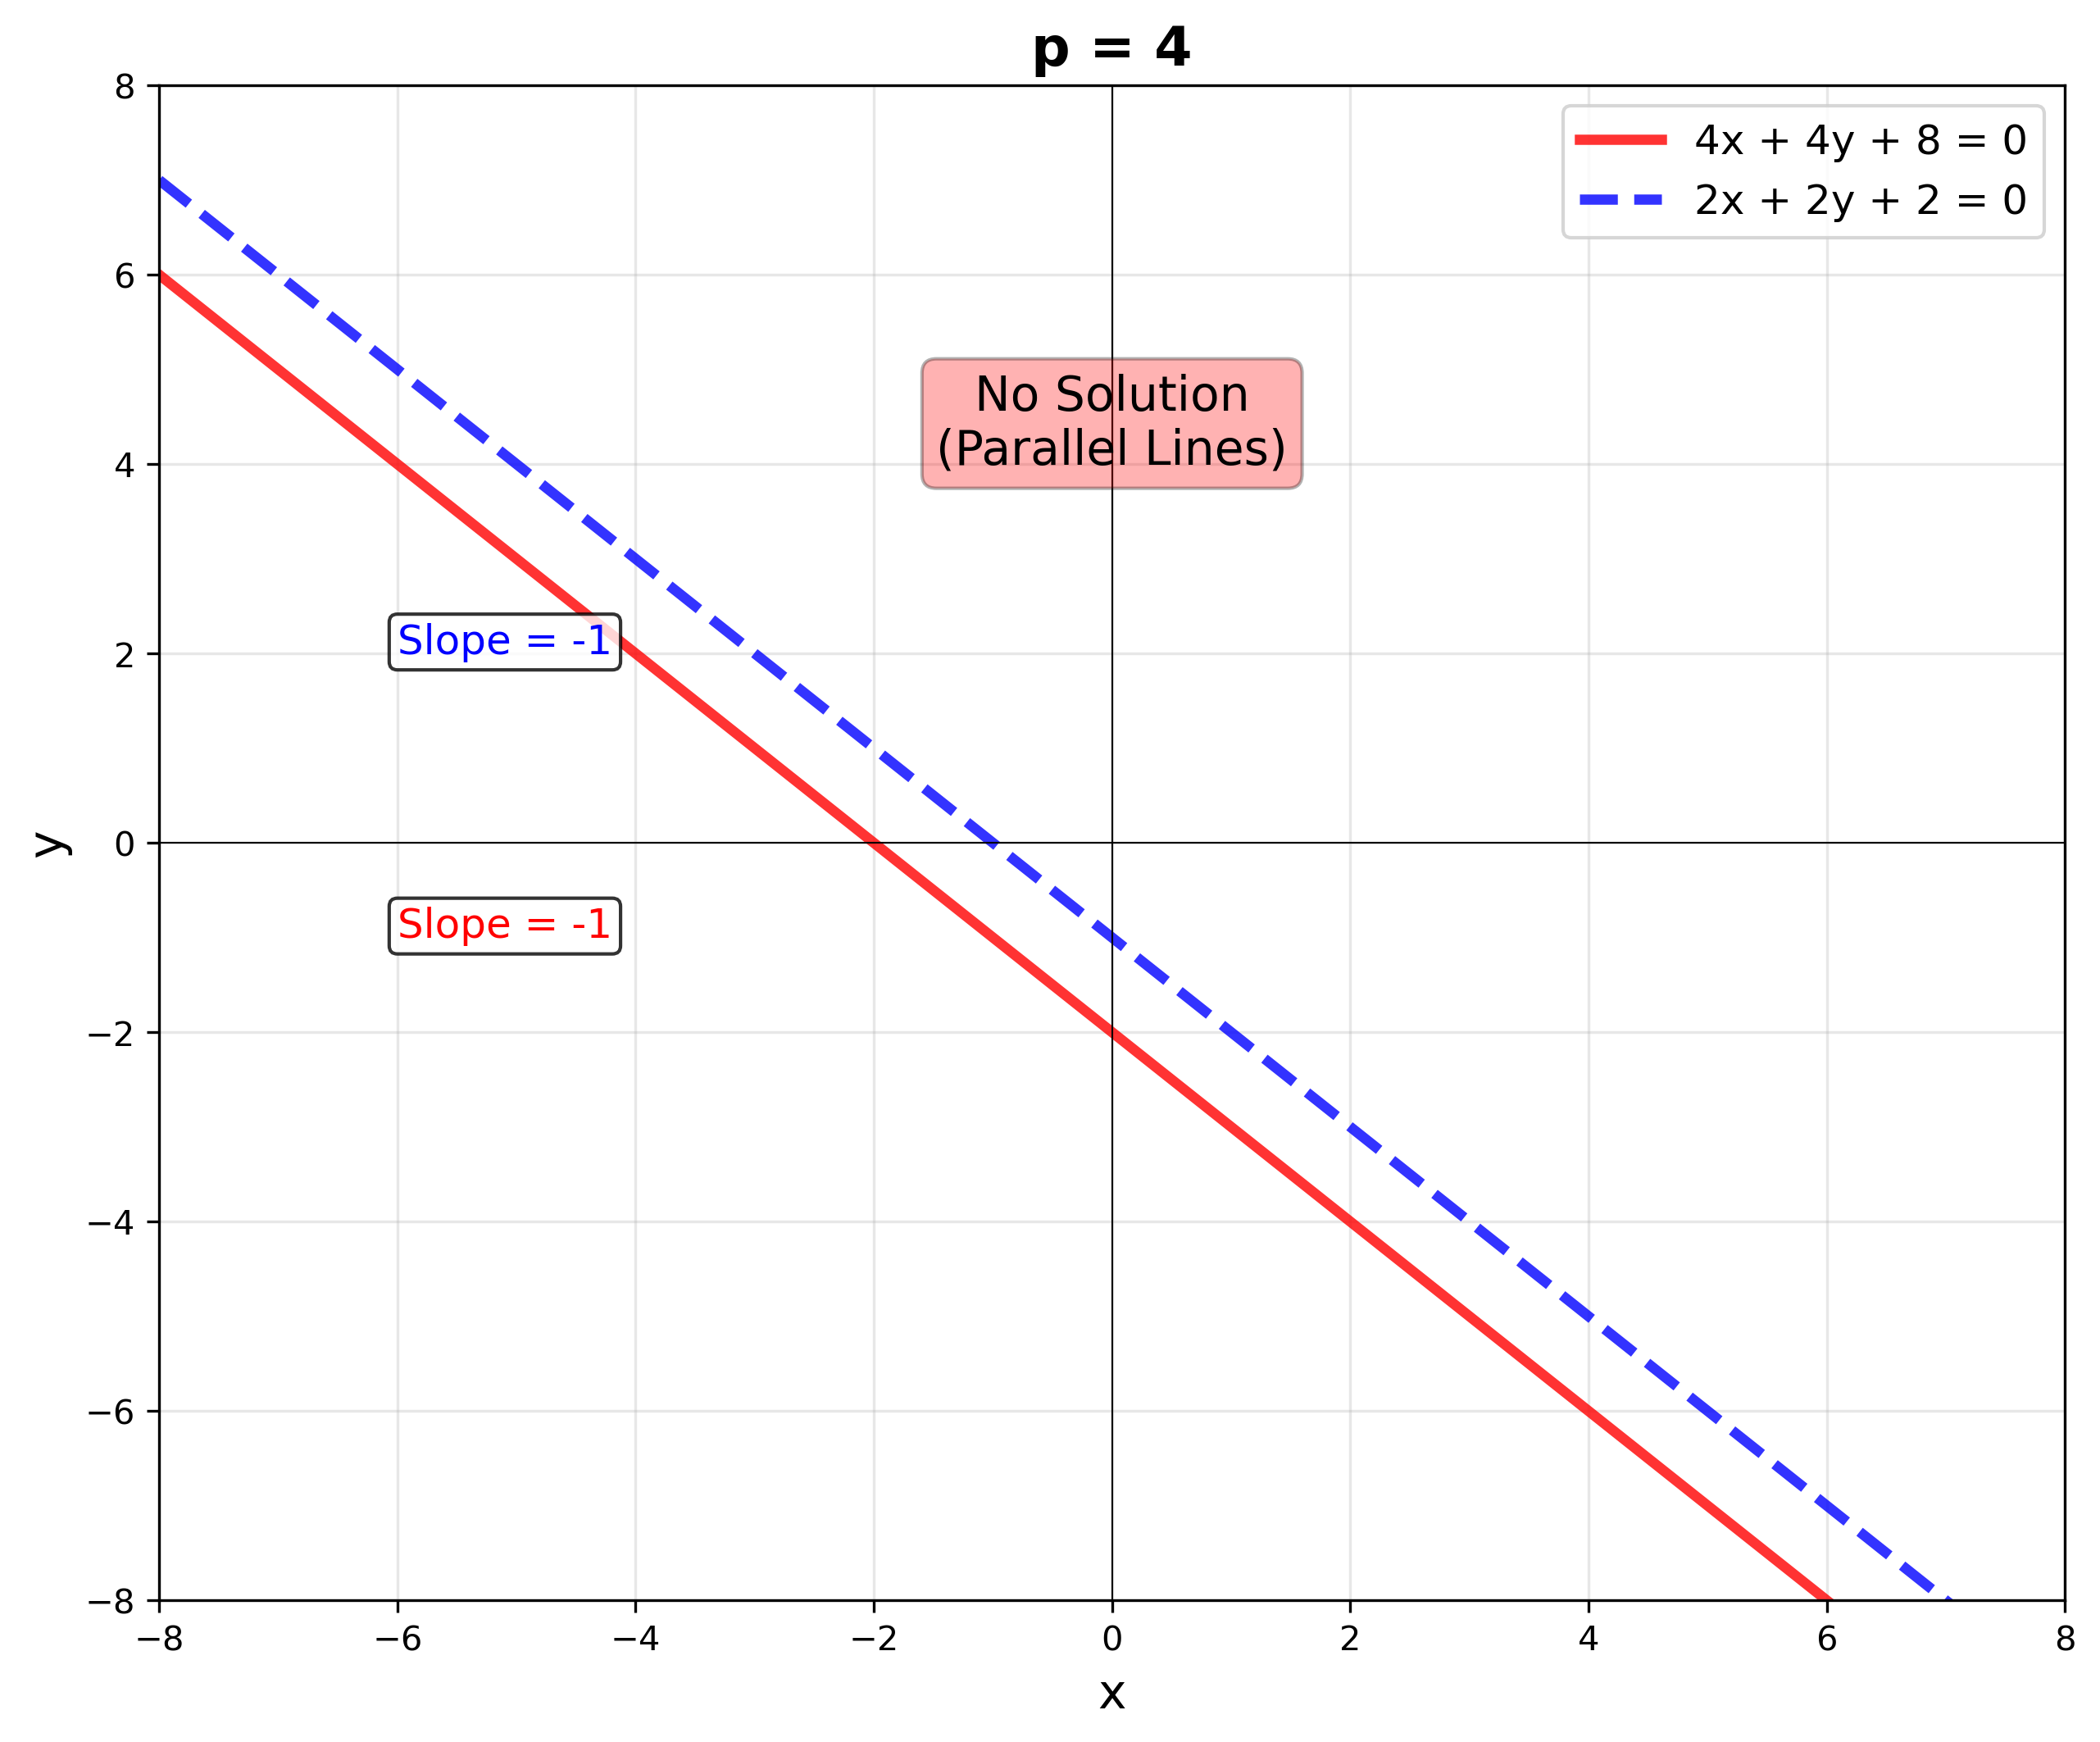
\includegraphics[width=0.7\columnwidth]{figs/fig1.png}
\label{fig:figs/fig1.png}
\end{figure}

\begin{figure}[htbp]
\centering
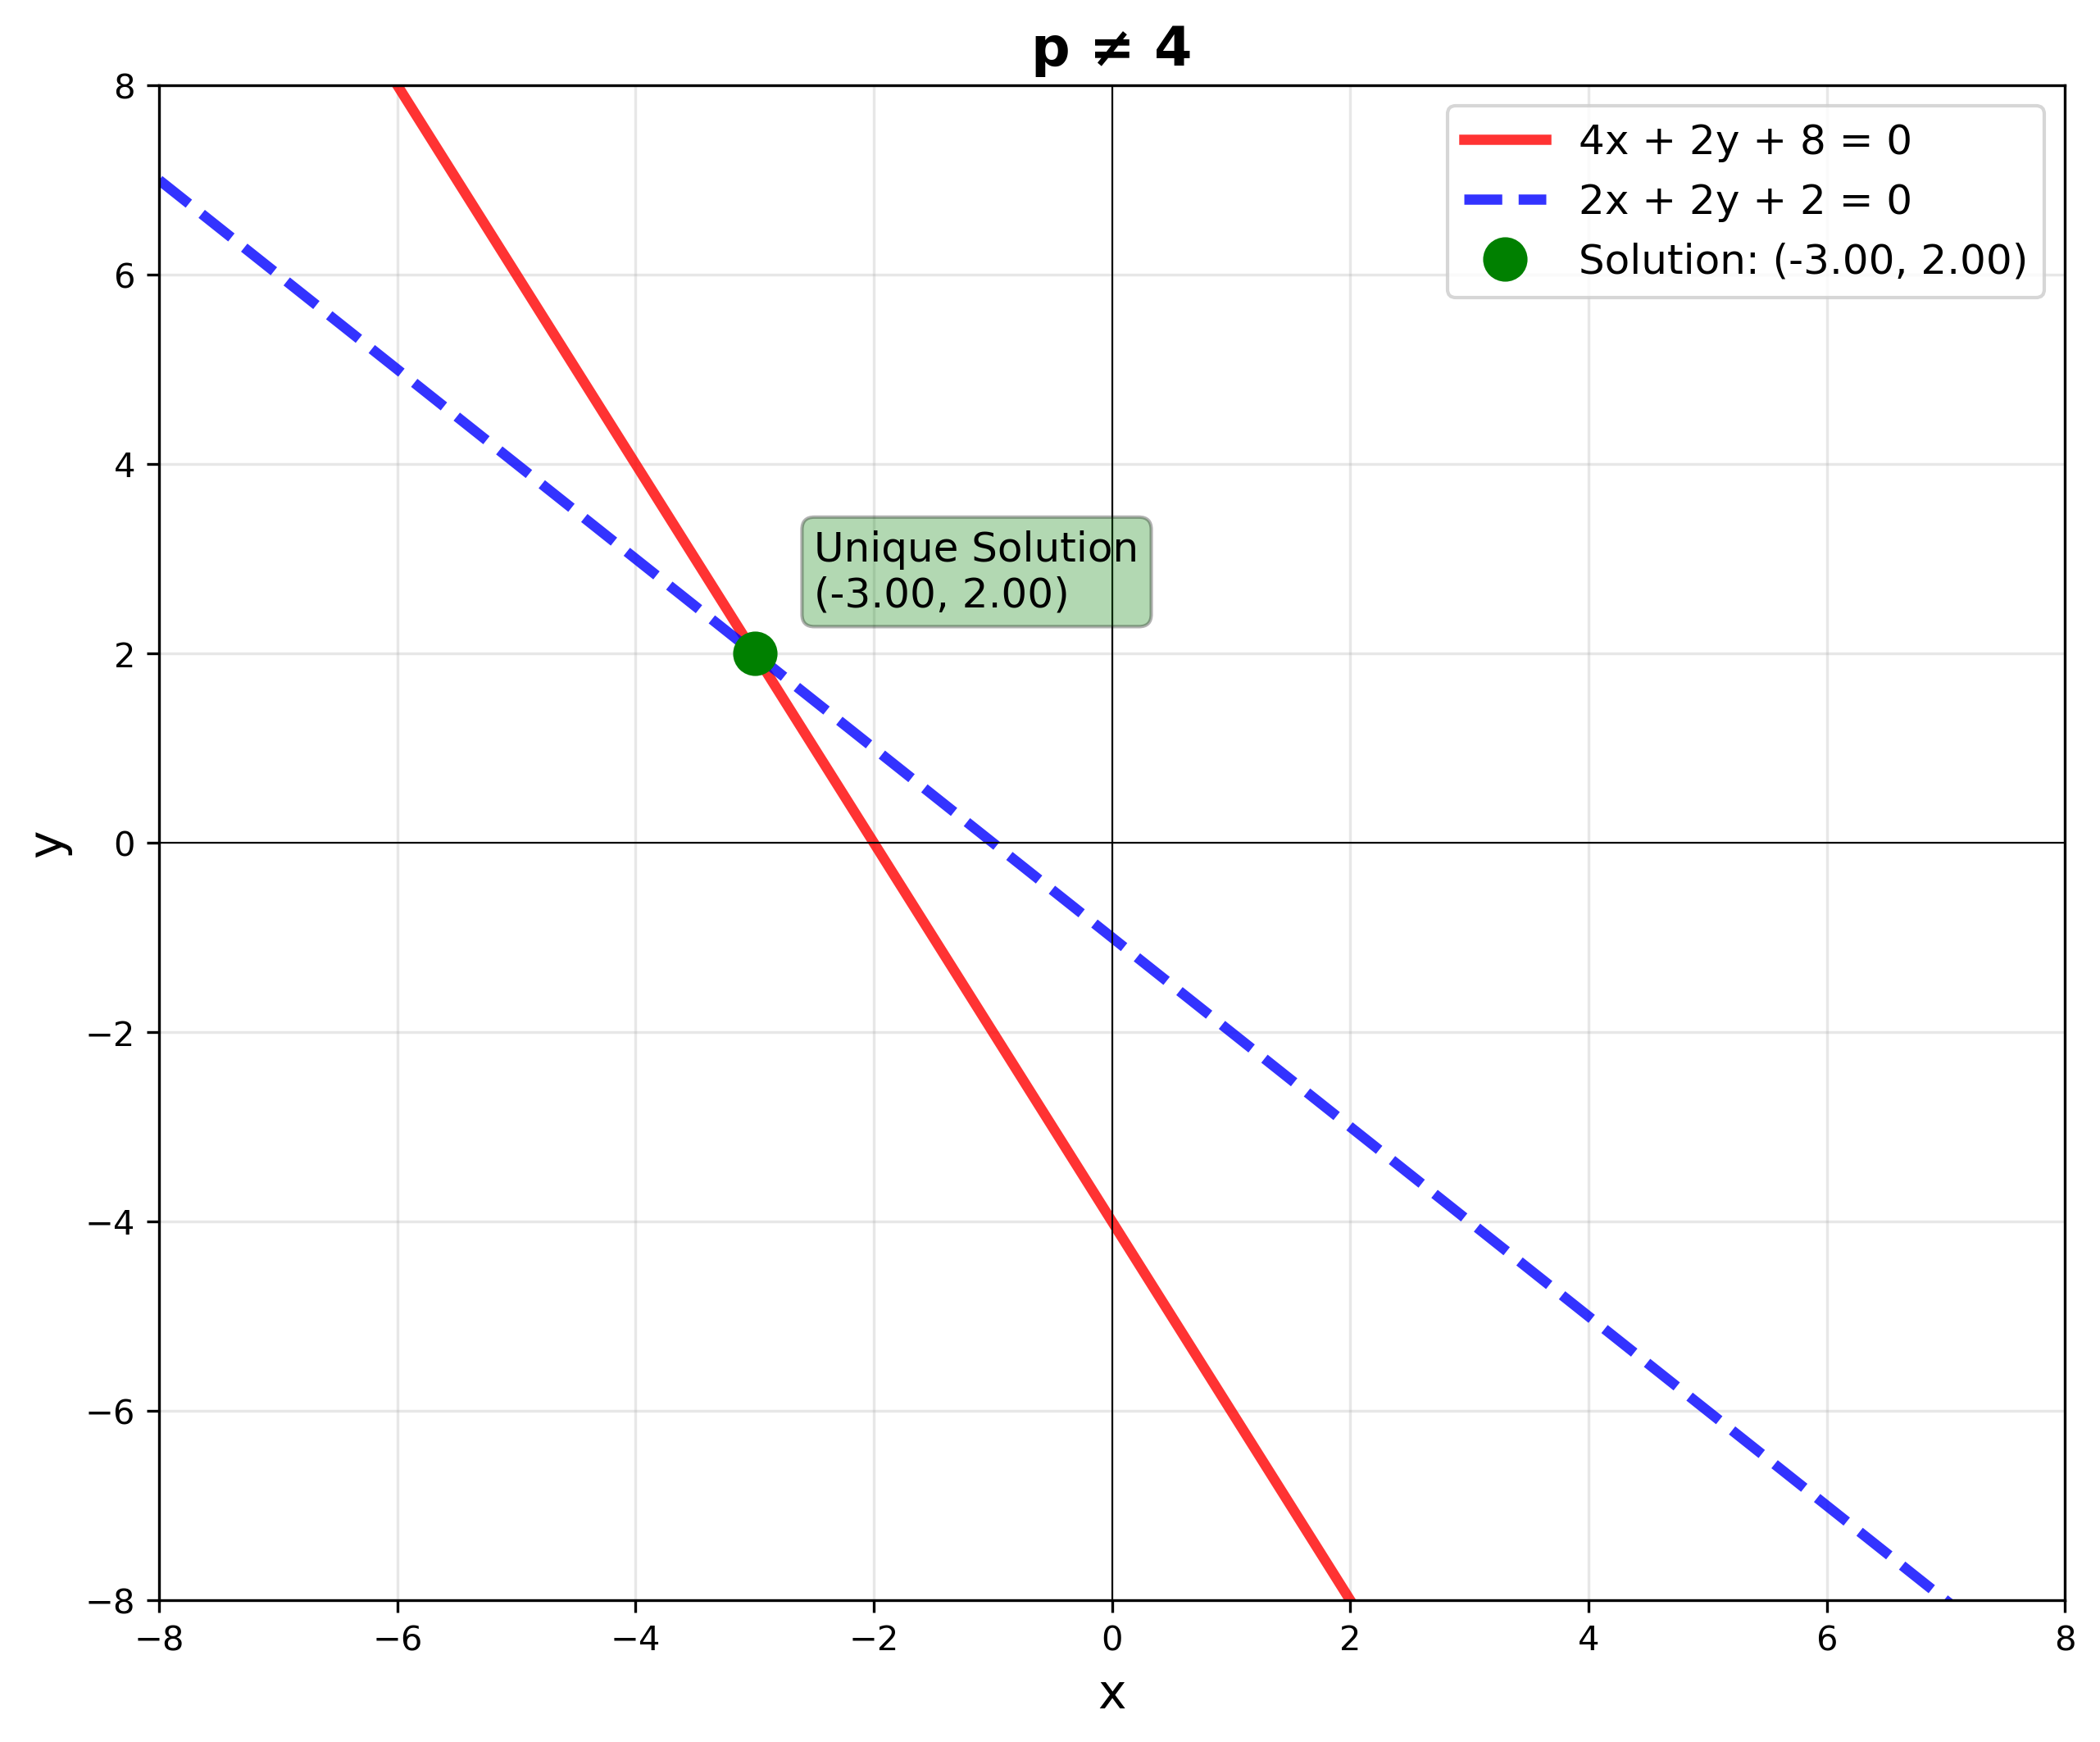
\includegraphics[width=0.7\columnwidth]{figs/fig2.png}
\label{fig:figs/fig2.png}
\end{figure}

\end{document}  
